\documentclass[a4paper]{report}

\usepackage[utf8x]{inputenc}
\usepackage{latexsym}
\usepackage[danish]{babel}
\usepackage{graphicx}
\usepackage{hyperref}
\usepackage[all]{hypcap}

\begin{document}
\title{En superkort introduktion til \LaTeX}

\author{Torben Mogensen}
\date{\today}

\maketitle

\begin{abstract}
I kurset ``Programmering og problemløsning'' (PoP) bruger vi
værktøjerne Emacs og \LaTeX.

Emacs er et tekstredigeringsværktøj, der er egnet til at redigere
programmer og lignende.  Et andet dokument introducerer Emacs. Ulig f.eks.\ Microsoft Word og Libre Office
Writer redigerer man med Emacs ``ren'' tekst: Der er ikke formatering
såsom fed skrift, kursiv, osv.  Til dette bruger vi \LaTeX.

\LaTeX\ (som udtales ``lahtek'') er et dokumentformateringsværktøj.
Det fungerer ligesom HTML ved, at man skriver formateringskoder ind i
en ren tekstfil, som derefter konverteres til et formateret dokument.
Hvor HTML konverteres i en browser til en webside, så konverteres
\LaTeX-dokumenter til PDF ved brug af værktøjet \texttt{pdflatex}.
\end{abstract}

\tableofcontents


\chapter{\LaTeX}

\LaTeX\ er et tekstformateringsværktøj designet til at skrive
strukturerede dokumenter såsom videnskabelige artikler, rapporter,
lærebøger, breve, Powerpoint-lignende præsentationer osv., men
\LaTeX\ kan også bruges til mange andre dokumentformer, for der er
rige muligheder for at definere sine egne strukturer og sit eget
layout.

\LaTeX\ udtales ``lahtek' og ikke ``lateks'', da de tre bogstaver i
\TeX\ faktisk er de græske bogstaver tau, epsilon og ksi, så denne del
af ordet udtales ``tech'' eller ``tek''. \LaTeX\ er en videreudvikling
af Donald Knuths \TeX\ lavet af Leslie Lamport, som satte bogstaverne
\textsf{La} foran navnet.  Det har altså intet med syntetisk gummi at
gøre, og vi \emph{har} allerede hørt alle vittighederne.

Den væsentligste forskel på \LaTeX\ og f.eks.~Microsoft Word er, at man
forbereder sine \LaTeX-dokumenter i et tekstredigeringsværktøj som
f.eks.~Emacs og derefter konverterer dem til PDF ved at køre et
program.  Det er i princippet ikke anderledes end den måde, et
HTML-dokument konverteres til tekst og billeder i et vindue i en
browser.  Et \LaTeX-dokument indeholder ud over den tekst, der skal
indgå i det færdige PDF-dokument, et antal koder og kommandoer, der
specificerer formatering, krydsreferencer, billedindsættelse,
formler, tabeller, figurer osv.  Det er \LaTeX-programmets opgave at
fortolke disse koder og bruge dem til at formatere dokumentets tekst.
Endvidere opdeler \LaTeX\ teksten i sider, som er egnede til
udskrivning, visning på en projektor, eller lignende, og indsætter
selv sidenumre osv.

\section{Installering af \LaTeX}

\LaTeX\ er gratis, open-source, og findes til en lang række platforme,
og der findes også web-værktøjer, hvor man kan lave \LaTeX-dokumenter
i sin browser.  Vi anbefaler, at man bruger Emacs på Linux, MacOS X
eller Windows til at redigere sine \LaTeX-dokumenter og derefter
konverterer dem til PDF med programmet \texttt{pdflatex}.  Her er en
meget kort instruktion til installering af dette program på de tre
hovedplatforme.

\paragraph{Linux.}

De fleste Linux-distributioner tillader installering af \LaTeX\ gennem
pakkesystemet, på samme måde som tidligere beskrevet for Emacs.  Vi
anbefaler, at du installerer \textsf{TeX Live}, der gør det nemt at
hente udvidelser osv.  Hvis du bruger Ubuntu Softwarecenter, så vælg
pakkerne \texttt{texlive-full} og \texttt{texlive-lang-all}.  Det
fylder en del, og det tager en del tid at hente, så sørg for at have
en god Internetforbindelse.

\paragraph{MacOs X.}

Vi anbefaler \textsf{MacTeX}, der indeholder \textsf{TeX Live} og et
par MacOS-specifikke udvidelser.  Den kan hentes på
\url{http://www.tug.org/mactex/}.

\paragraph{Windows.}

Følg instruktionen på\newline
\url{http://www.tug.org/texlive/acquire-netinstall.html}.

\section{Brug af \LaTeX}

For at afprøve installeringen af \LaTeX, anbefaler vi, at du starter
med et meget simpelt dokument.  Brug Emacs til at oprette en fil
\texttt{Hello.tex}, der indeholder følgende tekst:

{\small
\begin{verbatim}
\documentclass{report}

\begin{document}

Hello World

\end{document}
\end{verbatim}
}

\noindent
Vi kommer tilbage til, hvad de enkelte dele af filen betyder senere.

Når du har gemt filen, så kør følgende kommando i et
kommandolinjevindue: \texttt{pdflatex~Hello.tex}.  Du skulle gerne få
noget output i stil med dette på din skærm (detaljerne kan variere fra
system til system):

{\small
\begin{verbatim}
This is pdfTeX, Version 3.1415926-2.5-1.40.14 (TeX Live 2013/Debian)
 restricted \write18 enabled.
entering extended mode
(./Hello.tex
LaTeX2e <2011/06/27>
Babel <3.9h> and hyphenation patterns for 78 languages loaded.
(/usr/share/texlive/texmf-dist/tex/latex/base/report.cls
Document Class: report 2007/10/19 v1.4h Standard LaTeX document class
(/usr/share/texlive/texmf-dist/tex/latex/base/size10.clo))
No file Hello.aux.
[1{/var/lib/texmf/fonts/map/pdftex/updmap/pdftex.map}] (./Hello.aux) )<
/usr/share/texlive/texmf-dist/fonts/type1/public/amsfonts/cm/cmr10.pfb>
Output written on Hello.pdf (1 page, 11544 bytes).
Transcript written on Hello.log.
\end{verbatim}
}

\noindent
Hvis du ser i filkataloget, vil du se, at der er oprettet tre nye
filer: \texttt{Hello.aux}, \texttt{Hello.log} og \texttt{Hello.pdf}.
Sidstnævnte skulle gerne være et et-sides PDF-do\-ku\-ment med teksten
``Hello World''.  \texttt{Hello.aux} indeholder information, som
\LaTeX\ bruger til krydsreferencer og lignende, så det er ikke
interessant at læse indholdet af dette.  \texttt{Hello.log} indeholder
en masse information om kørslen af \LaTeX, som for det meste også er
uinteressant, men som kan bruges til at finde oplysninger om fejl.
Lad os tage et eksempel: Vi staver med vilje forkert i den sidste
linje:


{\small
\begin{verbatim}
\documentclass{report}

\begin{document}

Hello World

\end{dokument}
\end{verbatim}
}

\noindent
Nu får vi følgende uddata, når vi kører \texttt{pdflatex~Hello.tex}:

{\small
\begin{verbatim}
This is pdfTeX, Version 3.1415926-2.5-1.40.14 (TeX Live 2013/Debian)
 restricted \write18 enabled.
entering extended mode
(./Hello.tex
LaTeX2e <2011/06/27>
Babel <3.9h> and hyphenation patterns for 78 languages loaded.
(/usr/share/texlive/texmf-dist/tex/latex/base/report.cls
Document Class: report 2007/10/19 v1.4h Standard LaTeX document class
(/usr/share/texlive/texmf-dist/tex/latex/base/size10.clo)) (./Hello.aux)

! LaTeX Error: \begin{document} ended by \end{dokument}.

See the LaTeX manual or LaTeX Companion for explanation.
Type  H <return>  for immediate help.
 ...                                              
                                                  
l.6 \end{dokument}
                  
? 
\end{verbatim}
}

\noindent
Linjen, der starter med \texttt{LaTeX Error} forklarer, at der er en
fejl, og hvad \LaTeX\ tror, fejlen er.  Lidt længere nede er der en
indikation af linjenummeret (\texttt{l.6}) og en gengivelse af den
fejlbehæftede linje.  Til sidst står et spørgsmålstegn.  Tryk
\textsf{x} og \textsf{Enter} for at komme ud af \texttt{pdflatex}, der
nu skriver

{\small
\begin{verbatim}
No pages of output.
Transcript written on Hello.log.
\end{verbatim}
}

\noindent
Bemærk, at forekomsten af en fejl medfører, at der ikke produceres
nogen PDF fil.  Hvis der allerede findes en PDF fil, bliver denne
dog liggende uændret.

Hvis vi i stedet ændrer sidste linje til

{\small
\begin{verbatim}
\edn{document}
\end{verbatim}
}

\noindent
får vi følgende fejlmeddelelse (efter samme indledende tekst):


{\small
\begin{verbatim}
! Undefined control sequence.
l.6 \edn
        {document}
? 
\end{verbatim}
}

\noindent
Meddelelsen \verb|Undefined control sequence| betyder, at \LaTeX\ ikke
kender kommandoen \verb|\edn|.  Den viser dette ved at opdele den
fejlbehæftede linje der, hvor den har fundet fejlen.  Igen kan man
trykke \textsf{x} og \textsf{Enter} for at komme ud.

Der er flere mulige fejlmeddelelser, som nogen gange kan være
kryptiske. En beskrivelse af de hyppigst forekommende fejlmeddelelser, og
deres mest sandsynlige årsag, kan findes på
\url{http://en.wikibooks.org/wiki/LaTeX/Errors_and_Warnings}.  En mere
komplet liste kan findes på
\url{http://www.eng.fsu.edu/~dommelen/l2h/errors.html}.


\subsection{Syntaks}\label{syntaks}

Vi kan af ovenstående se, at ikke alle tekstfiler kan konverteres til
PDF af \texttt{pdflatex}: De skal opfylde nogle regler for tekstens
struktur.  Disse regler kaldes \emph{syntaks}, et begreb, der også
findes for ``rigtige'' sprog såsom dansk og engelsk.  Groft sagt
dækker begrebet syntaks de \emph{grammatiske regler og staveregler},
der kendetegner et skrevet sprog, men uden at tage hensyn til
\emph{betydningen} af den skrevne tekst.

Et \LaTeX\ dokument skal starte med kommandoen \verb|\documentclass|
efterfulgt af navnet på en dokumenttype indeholdt i krøllede
parenteser (kendt som ``mængdeparenteser'' i matematik).  I eksemplet
herover har vi brugt dokumenttypen \texttt{report}, som bruges til at
skrive rapporter.  Andre dokumenttyper er \texttt{article},
\texttt{book} og \texttt{letter}, som mere eller mindre siger sig
selv, og \texttt{beamer}, der bruges til Powerpoint-lignende
præsentationer.  Vi holder os primært til \texttt{report} i denne korte
vejledning.

Derefter kan komme et antal kommandoer, som man kalder
``indledningen'' (eller \emph{the~preamble}), hvorefter dokumentets
hovedindhold kommer omsluttet af kommandoerne \verb|\begin{document}|
og \verb|\end{document}|.  Al tekst efter dette vil blive ignoreret.
Vores ``Hello World'' eksempel er altså stort set et minimalt
\LaTeX-dokument.

Da \LaTeX\ er designet i USA, er standardindstillingerne, at PDF-filen
bruger det amerikanske letter-papirformat.  Dette format er en smule
bredere end A4, men ikke helt så højt.  For at få \LaTeX\ til at
producere PDF formateret til A4-papir, ændrer vi første linje til

{\small
\begin{verbatim}
\documentclass[a4paper]{report}
\end{verbatim}
}

\noindent
Man kan angive andre papirformater i stedet for A4, blandt andet
\texttt{a5paper} og \texttt{b5paper}.  Vi holder os dog til A4 papir,
da det passer til de fleste printere.  For at kunne bruge de danske
bogstaver æ, ø og å og accenter såsom é, for at få automatisk
orddeling tilpasset det danske sprog, og et par andre ting, som vi
kommer tilbage til senere, tilføjer vi et antal kommandoer til
indledningen, som dermed bliver

{\small
\begin{verbatim}
\documentclass[a4paper]{report}

\usepackage[utf8x]{inputenc}
\usepackage{latexsym}
\usepackage[danish]{babel}
\usepackage{graphicx}
\usepackage{hyperref}
\usepackage[all]{hypcap}
\end{verbatim}
}

\noindent
Du behøver ikke at forstå, hvad alle disse kommandoer betyder, men du
bør bemærke, at tegnene \verb|\|, \verb|{|, \verb|}|, \verb|[| og
\verb|]| bruges i kommandoer.  \LaTeX\ bruger yderligere et antal tegn
til kommandoer, så følgende tegn kan ikke uden videre bruges i
tekster, uden at \LaTeX\ måske fortolker dem som dele af kommandoer:

{\small
\begin{verbatim}
\ { } [ ] $ & # % ^ _ ~
\end{verbatim}
}

\noindent
Hvis man i sin tekst gerne vil bruge disse tegn, kan man i de fleste
tilfælde bare sætte et \verb|\| foran, så teksten \verb|\{\$\_\%\}|
producerer tegnfølgen \{\$\_\%\} i PDF-filen.  Der er dog undtagelser:
Tegnet $\backslash$~produceres med kommandoen \verb|$\backslash$|,
tegnet \~{} med kommandoen \verb|\~{}|, tegnet \^{} med kommandoen
\verb|\^{}|, og tegnene [ og ] kan uden videre skrives, som de er, så
længe de ikke kommer lige efter et kommandonavn.

Hvis man bruger disse tegn til andet end kommandoer, vil man enten få
fejlmeddelelser, eller man vil få et andet resultat, end det man
venter.  Specielt vil tegnet \verb|~| i reglen vises som et blanktegn,
og alle tegn mellem et \verb|%| og næste linjeskift ignoreres af
\LaTeX.  Dette kan man bruge til at skrive noter om ting, man gerne
vil skrive ind i dokumentet senere, f.eks.\

{\small
\begin{verbatim}
H.~C.~Andersen sagde »At rejse er at leve«.
% check lige, om citatet er rigtigt.
\end{verbatim}
}

\noindent
som blot giver outputtet

\begin{quote}
H.~C.~Andersen sagde »At rejse er at leve«.
\end{quote}

\noindent
Generelt vil \LaTeX\ samle gentagne blanktegn til et enkelt og betragte
linjeskift på lige fod med blanktegn.  Dog indikerer to eller flere
linjeskift efter hinanden, at et nyt tekstafsnit begynder.
F.eks.~giver teksten

{\small
\begin{verbatim}
Det   var   en mørk og
stormfuld
   nat.


Men intet
  interessant
skete.
\end{verbatim}
}

\noindent
outputtet

\vspace{1ex}
~\begin{tabular}{p{20em}}
Det   var   en mørk og
stormfuld
   nat.


~~~Men intet
  interessant
skete.
\end{tabular}

\vspace{1ex}

\noindent
Hvis man ønsker flere blanktegn efter hinanden i en tekst, kan man
bruge tegnet \verb|~| det nødvendige antal gange.  Man kan tvinge et
linjeskift med kommandoen \verb|\newline|.

Fordi linjeskift (enkeltvis) har samme betydning som blanktegn, anbefaler
vi, at man i Emacs bruger auto-fill-mode, når man skriver
\LaTeX\ dokumenter.

\section{Et struktureret dokument}

Som nævnt, fokuserer vi her på rapporter, indikeret af dokumentklassen
\texttt{report}.  Det er denne dokumentklasse, der er brugt til at
lave det dokument, du netop er i gang med at læse.

En rapport har en forside med en titel, en forfatter og en dato.
Forsiden laves ved at angive de relevante informationer med
kommandoer, og derefter lave forsiden med kommandoen
\verb|\maketitle|.  Titelsiden på indeværende
dokument er lavet med kommandoerne

{\small
\begin{verbatim}
\title{En superkort introduktion til \LaTeX}
\author{Torben Mogensen}
\date{\today}
\maketitle
\end{verbatim}
}

\noindent
der alle står lige efter \verb|\begin{document}|.  Kommandoerne
\verb|\title|, \verb|\author| og \verb|\date| siger sig selv.
Kommandoen \verb|\LaTeX| genererer \LaTeX-logoet, og \verb|\today|
indsætter dags dato i dokumentet.  Det er en god måde at sikre sig, at
datoen på forsiden faktisk svarer til den seneste udgave af
dokumentet.

En rapport består af kapitler (indledt med
\verb|\chapter{overskrift}|), der er opdelt i nummererede afsnit
(indledt med \verb|\section{overskrift}|), og underafsnit (indledt med
\verb|\subsection{overskrift}|).  \LaTeX\ finder selv ud af
nummereringen, man skal blot angive titlerne på kapitler og afsnit.  I
rapporter starter kapitler på nye sider, så \LaTeX-dokumentet vist i
figur~\ref{simple} vil generere to korte kapitler startende på hver
sin side.  Prøv selv at kopiere teksten ind i Emacs, gem den under
navnet \texttt{simple.tex}, og kør kommandoen
\texttt{pdflatex~simple.tex}.


\begin{figure}
\label{simple}

{\small
\begin{verbatim}
\documentclass{report}

\usepackage[utf8x]{inputenc}
\usepackage{latexsym}
\usepackage[danish]{babel}
\usepackage{graphicx}
\usepackage{hyperref}
\usepackage[all]{hypcap}

\begin{document}

\title{En kort rapport}
\author{Torben Mogensen}
\date{\today}
\maketitle

\chapter{Introduktion}

Dette er et eksempel på en simpel rapport.

\section{Formål}

Formålet er at vise, hvordan en simpel rapport struktureres i \LaTeX.

\section{Målgruppe}

Dokumentet retter sig mod studerende på kurset PoP.

\subsection{Hvad er PoP?}

PoP er en forkortelse for "Programmering og problemløsning".

\chapter{Konklusion}

Det er ikke svært, at få rapporter til at se professionelle ud, når
man bruger \LaTeX.

Ting lavet i Microsoft Word ser amatøragtigt ud i sammenligning.

\section{Videre arbejde}

Vi har kun dækket en brøkdel af, hvad man kan i \LaTeX, så vi
fortsætter straks med flere detaljer.

\end{document}
\end{verbatim}
}
\caption{Eksempel på simpel rapport i \LaTeX}
\end{figure}

Bemærk, at de første tekstafsnit i hvert kapitel eller afsnit ikke er
indrykket, mens de efterfølgende er.  Det ses i starten af kapitel 2.
Hvis man ikke ønsker, at et tekstafsnit skal indrykkes, kan man
indsætte kommandoen \verb|\noindent| på linjen lige inden
tekstafsnittet.  Det bruger man f.eks.~i tekstafsnit, der står lige
efter diagrammer eller formler, der vises på linjer for sig med blanke
linjer imellem.  Vi har i denne rapport blandt andet brugt det efter
de eksempler på input og output til \LaTeX, der står i
\texttt{skrivemaskineskrift}.

Til kortere dokumenter kan man bruge dokumentklassen \texttt{article}.
Her kan man ikke bruge kapitler (kommandoen \verb|\chapter|) er
udefineret, så man bruger \verb|\section| som hovedstruktur.  Der laves
ikke en separat titelside, så titel osv.\ placeres blot øverst på første
side.  Emacs-introduktionen er lavet med dokumentklassen \texttt{article}.

\section{Fed tekst, kursiv, m.m.}

\LaTeX\ finder selv ud af at skrive overskrifter på kapitler og afsnit
med fed og stor tekst, men man kan også selv fremhæve tekst ved at
gøre den kursiv eller fed.  Den anbefalede måde at fremhæve noget som
kursiv er med kommandoen \verb|\emph|, der er kort for
\emph{emphasize}.  Det sidste ord i den foregående sætning er
f.eks.~lavet med kommandoen \verb|\emph{emphasize}|.  Fed tekst laves
med kommandoen \verb|\textbf| (hvor \texttt{bf} står for
\textbf{boldface}).  F.eks.~er sidste ord i parentesen lavet med
kommandoen \verb|\textbf{boldface}|.  Skrivemaskinetekst laves med
kommandoen \verb|\texttt| (hvor \texttt{tt} står for
\texttt{teletype}, som er betegnelsen for en skrivemaskine, der styres
af en computer).  Du kan nok gætte, hvordan denne kommando bruges.

Når man vil vise programtekster, er det irriterende, at
\LaTeX\ ignorerer linje\-skift og gentagne blanktegn.  Derfor bruger
man f.eks.\ \texttt{verbatim} omgivelserne.  Omgivelser er en særlig
slags kommandoer, der typisk bruges til ting, der står på linjer for
sig selv i stedet for midt i en tekst.  I stedet for at skrive en
enkelt kommando med et argument i krølleparenteser, bruger man
kommandoen \verb|\begin| til at starte omgivelsen og \verb|\end| til
at afslutte den.  Vi har allerede set \verb|\begin{document}| og
\verb|\end{document}|, der er en en omgivelse for hele dokumentets
indhold.  Til programtekst kan vi skrive for eksempel

\vspace{2ex}
\noindent
{\small
\begin{tabular}{@{}l}
\verb|\begin{verbatim}|\\
\verb|let rec factorial n = |\\
\verb|    if n = 0 |\\
\verb|    then 1 |\\
\verb|    else n * factorial (n - 1)|\\
\verb|\end{verbatim}|\\
\end{tabular}
}
\vspace{2ex}

\noindent
Som vises som

{\small
\begin{verbatim}
let rec factorial n = 
    if n = 0 
    then 1 
    else n * factorial (n - 1)
\end{verbatim}
}

\noindent
Alle kommandoer mellem \verb|\begin{verbatim}| og
\verb|\end{verbatim}| ignoreres og vises blot som tekst.  Af denne
grund er \texttt{verbatim} omgivelserne brugt til at vise input og
output fra \LaTeX\ i dette dokument.

Der findes pakker til \LaTeX, der kan lave mere avanceret formatering
af programtekst, men dem gemmer vi til senere.

\section{Krydsreferencer og figurer}

En af de stærke sider ved \LaTeX\ er håndteringen af krydsreferencer.

Med kommandoen \verb|\tableofcontents| kan man generere en
indholdsfortegnelse. \LaTeX\ finder selv ud af at udfylde
indholdsfortegnelsen med de kapitler og afsnit, man har brugt i
rapporten.  Ved skærmlæsning, kan man følge link fra
indholdsfortegnelsen til de angivne kapitler og afsnit.  Hvis man
bruger \verb|\tableofcontents|, vil \texttt{pdflatex} oprette filer
med endelserne \texttt{.out} og \texttt{.toc}.  Lige som
\texttt{.aux}-filer, behøver man ikke at læse disse -- de bliver blot
brugt af \texttt{pdflatex} til at holde styr på tingene.

Hvis man i sin tekst vil lave en krydsreference til et andet kapitel
eller afsnit, bruger man kommandoerne \verb|\label| og \verb|\ref|.
\verb|\label| placeres ved den \verb|\chapter|, \verb|\section| eller
lignende kommando, der definerer det sted, man vil krydsreferere til,
og gives et navn som argument.  Jeg har f.eks.\ defineret
afsnit~\ref{supplerendeLatex} med kommandoerne

\begin{verbatim}
\section{Supplerende litteratur}\label{supplerendeLatex}
\end{verbatim}

\noindent
Dette gør, at jeg ved at skrive \verb|afsnit~\ref{supplerendeLatex}|
får krydsreferencen ``afsnit~\ref{supplerendeLatex}''.  Hvis den
genererede PDF fil læses på en skærm i stedet for papir, vil
krydsreferencen endvidere vises i en rød kasse, som er et link, man
kan følge med et museklik.  Hvis man bruger \verb|\ref| med et navn,
der ikke er defineret med en \verb|\label|-kommando, skriver
\LaTeX\ \textbf{??} i stedet for krydsreferencen, og \texttt{pdflatex}
skriver

\begin{verbatim}
LaTeX Warning: There were undefined references.
\end{verbatim}

\noindent
Dette kan også ske, hvis man refererer til en label længere fremme i
teksten, men det løses ved at køre \texttt{pdflatex} en gang til.

Krydsreferencer bruges også til at henvise til figurer,
f.eks.\ figur~\ref{simple}.  En figur defineres med omgivelsen
\texttt{figure} og gives en titel med kommandoen \verb|\caption|.  En
figur kan f.eks.\ defineres med kommandoerne

\begin{verbatim}
\begin{figure}\label{eksempelfigur}

\begin{center}
Dette er indholdet af figuren.
\end{center}

\caption{Eksempel på figur}

\end{figure}
\end{verbatim}

\begin{figure}\label{eksempelfigur}

\begin{center}
Dette er indholdet af figuren.
\end{center}

\caption{Eksempel på figur}

\end{figure}

\noindent
som genererer figur~\ref{eksempelfigur}.  Figurer nummereres og
placeres automatisk.  Normalt vil \LaTeX\ placere en figur øverst
eller nederst på en side eller på en side for sig i stedet for midt på
en side.  Den vil aldrig komme på en side før det sted, hvor
kommandoen er placeret, men det kan godt være flere sider senere.

Andre former for krydsreferencer er links til websider og fodnoter.
Et link til en webside skrives med kommandoen \verb|\url|,
f.eks.\ \verb|\url{http://www.diku.dk}|, der genererer følgende URL:
\url{http://www.diku.dk}.  Når dokumentet læses på en skærm, kan man
følge linket med et museklik.

En fodnote
skrives med kommandoen \verb|\footnote|.  Fodnoten nederst på denne
side\footnote{Ja, denne fodnote} er lavet med kommandoen
\verb|\footnote{Ja, denne fodnote}| lige efter ordet ``side''.

En mere avanceret form for krydsreference er en litterær henvisning.
\LaTeX\ har et værktøj kaldet {\small BIB}\TeX, der gør dette nemt.
Vi henviser til den supplerende litteratur i
afsnit~\ref{supplerendeLatex} for detaljer om, hvordan man bruger
{\small BIB}\TeX. .

\section{Formler}

\LaTeX\ er særlig god til at skrive matematiske formler.  Vi har ikke
plads her til at dække alle former for formler, så vi holder os til
det simple.  En formel kan skrives enten inde i et tekstafsnit eller
på en linje for sig, hvor den bliver centreret og omgivet af blanke
linjer.  Se f.eks.\ forskellen på $ax^2+bx+c=0$ og

\[ax^2+bx+c=0\]

\noindent
Formler inde i tekstafsnit omgives af dollartegn, så den viste formel
skrives som \verb|$ax^2+bx+c=0$|.  For at få formlen på en linje for
sig, omgives den af \verb|\[| og \verb|\]|, altså
\verb|\[ax^2+bx+c=0\]|.

Som det kan ses, laves hævet tekst i formler ved at sætte tegnet
\verb|^| foran.  Dette vil kun løfte et enkelt tegn, men man kan sætte
krølleklammer rundt om flere tegn for at få dem alle løftet.  For
eksempel vil teksten \verb|$e^{-x}$| give formlen $e^{-x}$, mens
teksten \verb|$e^-x$| giver formlen $e^-x$.  Sænket tekst laves
tilsvarende med \verb|_|, så \verb|$x_0$| giver formlen $x_0$.  De kan kombineres, så \verb|$x_0^n$| giver $x_0^n$.

Generelt bliver blanktegn ignoreret i formler, så \verb|$a bc$| vises
som $a bc$.  Man kan dog sætte et \verb|~| ind, hvis man vil have et
blanktegn.  Som det ses af eksemplerne, vises bogstaver i kursiv i
formler, men matematiske funktioner som $\log$ og $\sin$ skrives
normalt med normal tekst i formler.  \LaTeX\ kender de fleste
matematiske funktioner, og man kan få dem til at se rigtige ud ved at
sætte et backslash foran.  Sammenlign \verb|$sin(x)$|, der giver
$sin(x)$, med \verb|$\sin(x)$|, der giver $\sin(x)$.  Græske bogstaver
skrives også med et backslash foran, så \verb|$\alpha\beta\Gamma$|
giver $\alpha\beta\Gamma$.  Bemærk, at vi fik et stort gamma, da vi
skrev \verb|Gamma| med stort begyndelsesbogstav.

\LaTeX\ kan også lave mere avancerede formler med integraler, brøker
og meget mere, f.eks.

\[\int_{x=0}^\infty{\frac{\log(x)}{x^2} dx}\]

\noindent
men vi henviser til supplerende litteratur i
afsnit~\ref{supplerendeLatex} for de mere avancerede dele.

\section{Billeder}

Man kan inkludere billeder i sin tekst med kommandoen
\verb|\includegraphics|, For eksempel er billedet af Emacs-skærmen i
Emacs-introduktionen lavet med kommandoen
\verb|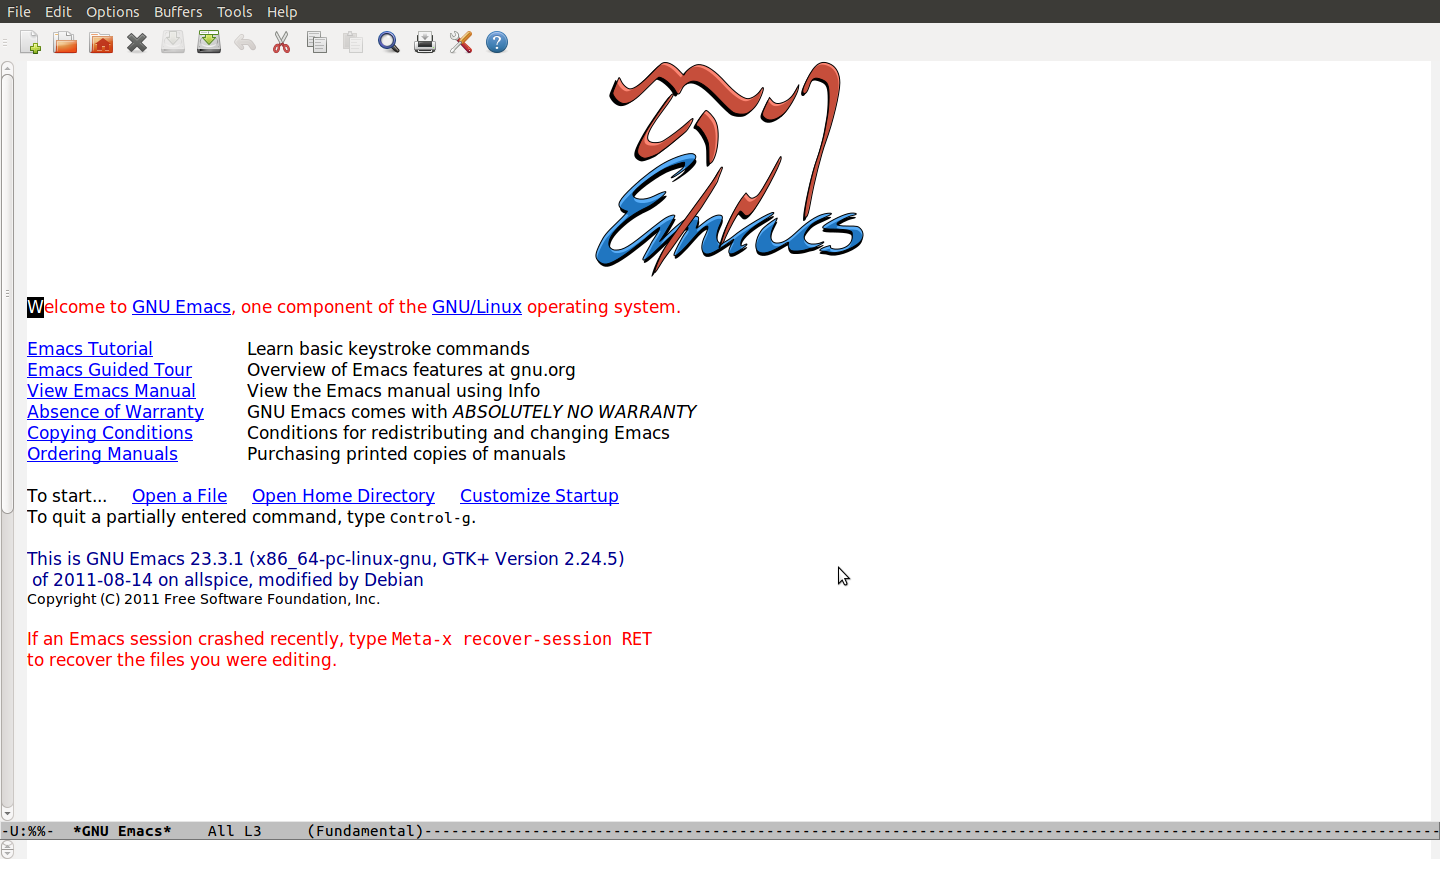
\includegraphics[width=\textwidth]{emacs-welcome.png}|. hvor\newline
\texttt{emacs-welcome.png} er en fil, der indeholder billedet i
billedformatet PNG.  Breddeangivelsen skalerer billedet til bredden af
teksten, idet \verb|\textwidth| angiver denne bredde.  Man kan også
angive bredde i f.eks.\ centimeter og millimeter, så kommandoen
\verb|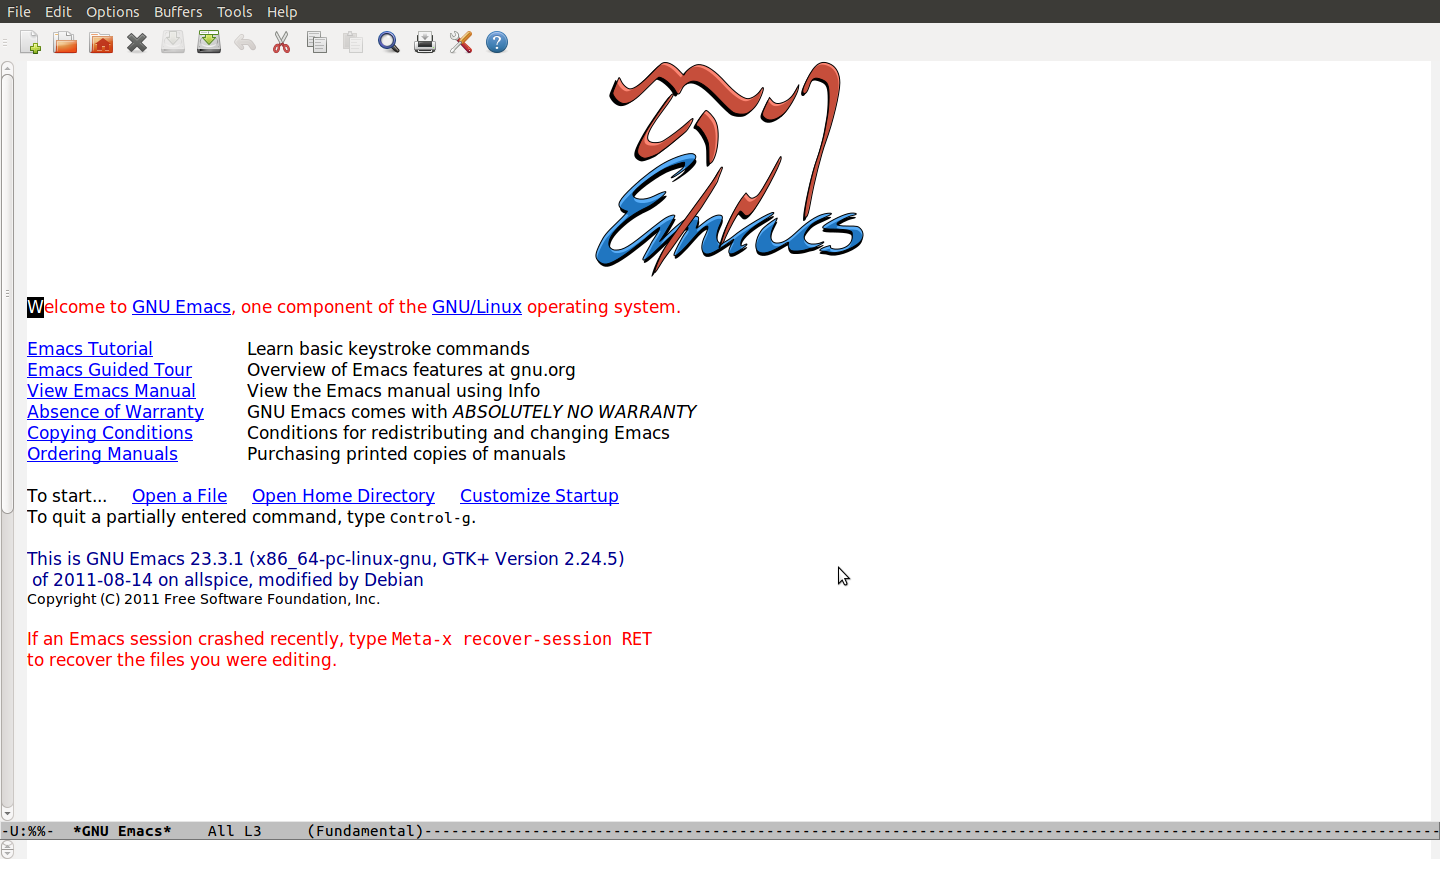
\includegraphics[width=5cm]{emacs-welcome.png}| vil skalere
billedet til en bredde på 5 centimeter.  Udover PNG kan
\texttt{includegraphics} også indlæse JPG og PDF.

Man kan centrere billeder (og andet) med \texttt{center} omgivelserne,
altså som f.eks.

\begin{verbatim}
\begin{center}
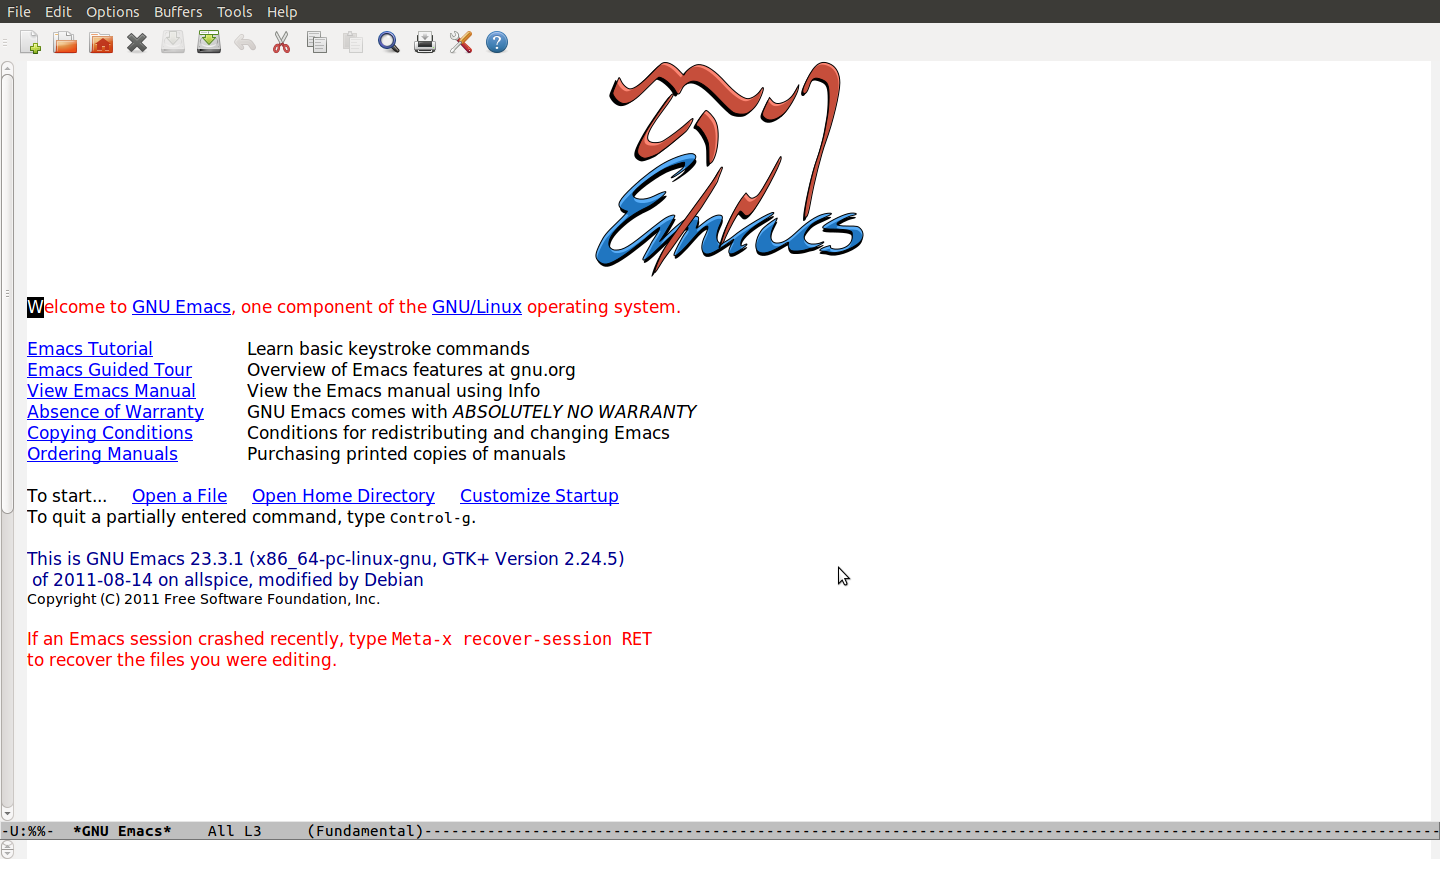
\includegraphics[width=5cm]{emacs-welcome.png}
\end{center}
\end{verbatim}

\noindent
som vil give dette resultat:

\begin{center}
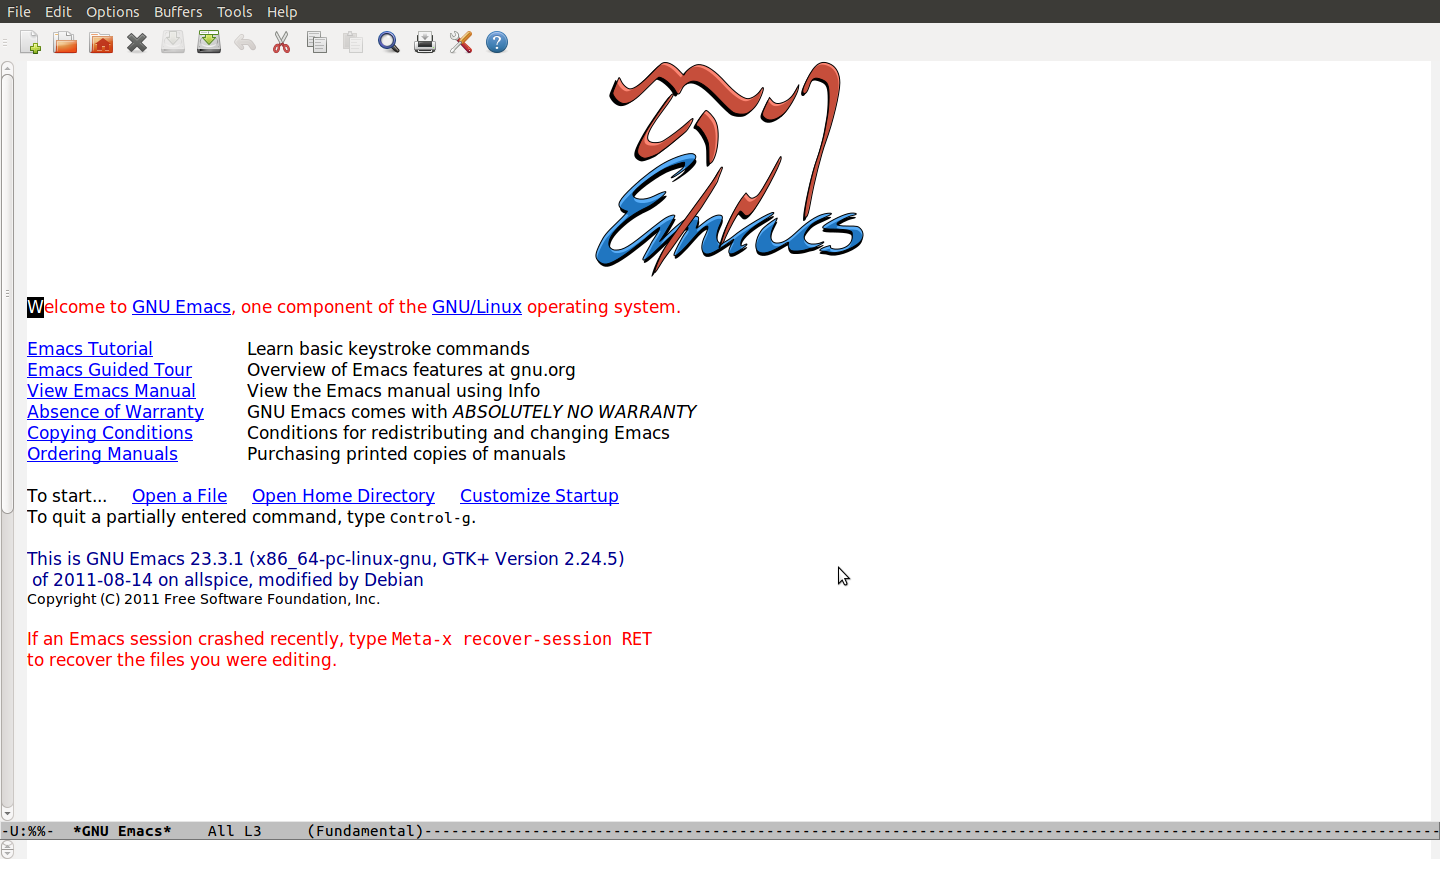
\includegraphics[width=5cm]{emacs-welcome.png}
\end{center}

\section{Udvidelsespakker}

Vi viste i afsnit~\ref{syntaks} en dokumentindledning med en række
\verb|\usepackage| kommandoer.  Denne kommando bruges til at tilføje
udvidelsespakker til den grundlæggende \LaTeX.  De viste pakker gør
følgende:

\begin{description}
\item[\texttt{$\backslash$usepackage[utf8x]\{inputenc\}}] tillader
  danske bogstaver og andre symboler i input.
\item[\texttt{$\backslash$usepackage\{latexsym\}}] udvider udvalget af
  matematiske symboler.
\item[\texttt{$\backslash$usepackage[danish]\{babel\}}] betyder, at
  visse autogenererede tekster (f.eks. ``Resumé'', ``Indhold'' og
  ``Kapitel'') skrives på dansk, sørger for at ord deles efter
  (tilnærmede) danske regler, skriver datoer (\verb|\today|) på dansk,
  og lignende sprogspecifikke ting.  Findes til de fleste sprog.
\item[\texttt{$\backslash$usepackage\{graphicx\}}] tillader indsætning
  af billeder med \verb|\includegraphics| kommandoen.
\item[\texttt{$\backslash$usepackage\{hyperref\}} og 
\texttt{$\backslash$usepackage[all]\{hypcap\}}] gør krydsreferencer
  til links.
\end{description}

\noindent
Der findes tusindvis af pakker til \LaTeX.  \textsf{TeX Live} sørger
for at hente de mest brugte pakker ved installering og henter flere
automatisk efter behov.  Nogle brugbare pakker er

\begin{description}
\item[listings] bruges (som alternativ til \texttt{verbatim}) til at
  vise programtekster.
\item[makeidx] bruges til at lave stikordslister.
\item[color] bruges til at lave farvet tekst.
\item[geometry] bruges til at ændre størrelsen af margener, papir,
  osv.
\item[fontenc] bruges til at indkode skriftsnit.  
  \verb|\usepackage[T1]{fontenc}| tillader PostScript type-1
  skriftsnit.
\item[cmap] Gør teksten i producerede PDF-filer søgbar og kopierbar.
  Bør komme før \texttt{fontenc} og \texttt{babel} i indledningen.
\end{description}

\noindent
Websiden \url{https://www.ctan.org/} er et arkiv over pakker til
\LaTeX, og man kan finde beskrivelser og vejledninger til over 5000
pakker på denne side.  Man kan søge efter navn eller emne.  Hvis man
f.eks.\ går ind i emnelisten under ``music'', finder man 35 pakker til
formatering af noder, guitarakkorder, sanghæfter, osv.

\section{\LaTeX\ og Emacs}

Emacs har en \LaTeX-mode, der blandt andet viser kommandonavne i
farver og viser kursiv og fed tekst som sådan.  Hvis man har
\LaTeX-mode installeret i sin Emacs, skifter Emacs automatisk til
denne mode, når man redigerer i en fil med filendelsen \texttt{.tex}.

\LaTeX-mode tilføjer et par \LaTeX-specifikke kommandoer til Emacs:
\textsf{C-c C-e} tilføjer en \verb|\end{}|-kommando svarende til den
nærmeste uparrede \verb|\begin{}|-kommando, og \textsf{C-c C-o}
tilføjer et par af \verb|\begin{}| og \verb|\end{}|-kommandoer, hvor
man kan vælge navnet ved at skrive det i minibufferen.

I \LaTeX-mode har Emacs også en TeX-menu, der blandt andet kan køre
kommandoen \texttt{latex} på den fil, man redigerer i, og vise
resultatet i et andet vindue.  Denne kommando producerer dog ikke PDF,
men et andet format, der hedder DVI, så selv om det er fint at bruge
denne menufunktion til at finde fejl i sit dokument, så bør man bruge
kommandoen \texttt{pdflatex} til sidst for at få output i PDF.
Endvidere kan \texttt{latex}-kommandoen ikke håndtere billeder i de
samme formater som \texttt{pdflatex}.

\section{Finpudsning}

Der er et par småting, men skal være opmærksom på, når man bruger
\LaTeX, så man får det pænest mulige resultat:

\begin{itemize}
\item Blanktegn lige efter en kommando, der ikke har parametre i
  krølleklammer, ignoreres.  For eksempel vil teksten
  \verb|\LaTeX styrer!| give resultatet {\LaTeX styrer!}  For at få et
  blanktegn ind alligevel give kommandoen en tom parameter, altså
  \verb|\LaTeX{} styrer!|, som giver resultatet {\LaTeX\ styrer!}.
  Det er ikke nødvendigt, hvis kommandoen følges af andet end
  blanktegn eller linjeskift, som f.eks.\ punktum eller komma.
  Alternativt kan man skrive \verb|\LaTeX\ styrer!|, altså sætte et
  backslash før blanktegnet, så det ikke bliver undertrykt.
\item Som det ses herover, kan \LaTeX\ nogen gange lade tekst strække
  sig ud over højre kant af tekst med lige højremargen.  Hvis dette
  sker, vil \texttt{pdflatex} give beskeden \verb|Overfull \hbox|, men
  ikke standse.  Denne besked er en \emph{advarsel} og ikke en
  \emph{fejlmeddelelse}, da den netop ikke hindrer produktion af
  output.  Efter beskeden \verb|Overfull \hbox|, angives hvor meget,
  teksten strækker sig ud, i dette tilfælde
  \verb|(24.74678pt too wide)| samt en angivelse af, hvor i teksten,
  dette forekommer.  Forkortelsen \verb|pt| står for ``punkt''; som er
  en typografisk måleenhed, der er ca.\ 0.35mm, så 24.74678pt er
  ca.\ 8.66mm.  I det viste tilfælde hjælper det at sætte \verb|{}|
  efter \verb|\LaTeX|, men i andre tilfælde kan man sætte kommandoen
  \verb|\newline| før det ord, der er for langt.  \LaTeX\ forsøger
  selv at dele ord efter regler for dansk orddeling, men hvis den er i
  tvivl, lader den være.  Hvis man får et langt ord, der stikker ud
  til højre, kan man hjælpe \LaTeX\ med orddelingen ved at sætte et
  \verb|\-| det sted, man gerne vil have delt ordet. \LaTeX\ vil kun
  indsætte en bindestreg, der hvor ordet deles (hvis det deles), så
  man kan sagtens indsætte flere for at give \LaTeX\ nogle
  valgmuligheder, f.eks.\ \verb|ord\-de\-ling|.

  Man kan også bruge \verb|\-|, hvis \LaTeX\ laver en forkert
  orddeling.  \LaTeX\ bruger et antal tommelfingerregler til
  orddeling, og det går nogle gange galt.  F.eks.\ vil \LaTeX\ dele
  ordet ``menupunkt'' som ``men-upunkt'', hvilket ikke er særligt
  kønt.  For at hindre dette, kan man skrive \verb|menu\-punkt|, som
  fortæller, at ordet kun må deles der.

  Lad dog være med at bekymre dig om forkert orddeling eller lige
  højrekant indtil du er færdig med at skrive rapporten: Det kan
  sagtens være, at du skriver om i teksten, så det ikke længere er et
  problem, og så er det spildt arbejde at bruge tid på orddeling eller
  tvungne linjeskift.

\item Der er forskel på bindestreger (-) og tankestreger (--).
  Bindestreger bruges til at dele ord og til visse ordsammensætninger
  -- f.eks.\ IT-sikkerhed -- og tankestreger bruges til indskud, som
  vist lige før.  En tankestreg skrives i \LaTeX\ som to bindestreger
  efter hinanden, altså \verb|--|.

\item \LaTeX\ skifter aldrig linje mellem ord, der er adskilt kun af
  \verb|~|.  Derfor kan man bruge dette tegn til at forhindre
  linjeskift mellem to ord.  Det kan f.eks.\ bruges til at forhindre et
  linjeskift mellem ``kapitel'' og ``2'' i ``kapitel~2''.

\item \LaTeX\ laver lidt større mellemrum efter et punktum, der
  afslutter en sætning, end efter f.eks.\ et komma.  Den måde,
  \LaTeX\ ser, om et punktum afslutter en sætning, er lidt primitiv:
  Hvis punktummet står lige efter et stort bogstav, tror \LaTeX, at der
  er tale om et forkortet navn, f.eks.\ H. C. Andersen, men hvis det
  kommer efter et lille bogstav, tror \LaTeX, at det er slutningen af
  en sætning.  For det meste fungerer dette fint, men efter
  forkortelser som f.eks.\ ``f.eks.'' er det forkert.  Man kan undgå
  det lange mellemrum efter en forkortelse ved at skrive en backslash
  lige efter punktummet, som f.eks.\ \verb|f.eks.\ H. C. Andersen|\@.
  Modsat kan man sætte \verb|\@| mellem et stort bogstav og et
  punktum, hvis man gerne vil have, at der kommer ekstra plads efter
  punktummet.  Det bruges hvis man afslutter en sætning med en
  forkortelse, der består af store bogstaver, som f.eks.\ DVD\@.  Den
  foregående sætning er f.eks.\ afsluttet med \verb|f.eks.\ DVD\@.|
\end{itemize}

\section{Supplerende litteratur}\label{supplerendeLatex}

Der findes mange vejledninger til \LaTeX\ på forskellige niveauer.  En
almindelig brugt vejledning er ``The Not So Short Introduction to
\LaTeX2$\varepsilon$'', som findes på
\url{https://tobi.oetiker.ch/lshort/lshort.pdf}.  Den kan virke lidt
uoverkommelig ved første øjekast, men den er god som oplagsværk.

Lidt mere tilgængelig er den \LaTeX\ tutorial, der ligger på
\url{http://www.latex-tutorial.com/tutorials/}.

Der findes en meget omfattende bog om \LaTeX\ på dansk, skrevet af Leif
Madsen fra Aarhus Universitet.  Den kan hentes på\newline
\url{http://math.au.dk/videnudveksling/latex/bog/}.

\section{Fortvivl ikke!}

\LaTeX\ kan i starten virke uoverskueligt, men man vænner sig hurtigt
til at bruge det, og efter nogen tid, vil man sætte pris på dets
muligheder.  Ældre studerende kan i reglen hjælpe dig, hvis du har
spørgsmål om \LaTeX, og hvis alt andet fejler, er Google din ven.

%Hvis man læser lærebøger og videnskabelige artikler indenfor datalogi
%og matematik, er de næsten altid lavet med \LaTeX, dels fordi det
%giver et bedre resultat end f.eks.\ Word og dels fordi konferencer og
%lærebogsforlag foretrækker at få artikler og bøger i \LaTeX.  Men selv
%om du ikke har planer om en akademisk karriere, bør du lære \LaTeX:
%Det gør dine rapporter pænere, og med tiden vil du opdage, at de
%faktisk også bliver nemmere at skrive.

\end{document}

